\begin{frame}{Motivační příklad: psaní I a Y (1)}

    \begin{columns}[t]
        \column{.48\textwidth}
        {\large\bf Jednoduchá pravidla} \\ ~

        \vspace{10pt}

    \begin{tabular}{lc}
        \visible<2->{
        & \bf Úspěšnost \\ \midrule
        Všechna I měkká        &    76.4\% \\}
        \visible<3->{
        + tvrdé souhlásky     &    77.5\% \\}
        \visible<4->{
        + předpona \emph{vy-} &    80.0\% \\}
    \end{tabular}

        \vspace{10pt}
        \visible<5->{Další pravidla potřebují větný rozbor}

        \column{.48\textwidth}
        \visible<6->{
            {\large\bf Jednoduchá statistika} \\}
        \visible<7->{
            \ldots každé slovo nejčastější pravopis}

        \vspace{10pt}

    \visible<8->{
    \begin{tabular}{rc}
        \bf Počet přečtených vět  &  \bf Úspěšnost \\ \midrule
                          500 &    77.9\% \\
                        5 000 &    85.3\% \\
                       50 000 &    88.6\% \\
                      500 000 &    90.4\% \\
                    5 000 000 &    90.8\% \\
    \end{tabular}}

    \end{columns}

    \vspace{20pt}

    {\tiny Zdroj: Jindřich's Blog \url{https://jlibovicky.github.io/2017/02/22/Pravopis.html}}

\end{frame}

% ----------------------------------------------------------------------------

\begin{frame}{Motivační příklad: psaní I a Y (2)}

    \centering
    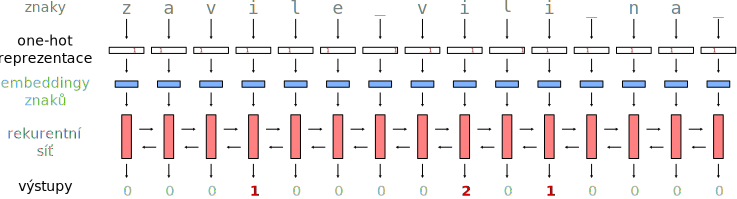
\includegraphics[scale=.65]{./img/cs_spelling.pdf}

    \visible<2->{
    \begin{columns}
        \column{.35\textwidth}
        \begin{tabular}{lc}
        \bf Metoda & \bf Úspěšnost \\ \midrule

        Všechna měkká        &    70.4 \% \\
        Jednoduchá pravidla  &    80.0 \% \\
        Nejčastější pravopis &    90.8 \% \\
        Neuronová síť        &    99.8 \% \\
        \end{tabular}

        \column{.45\textwidth}
        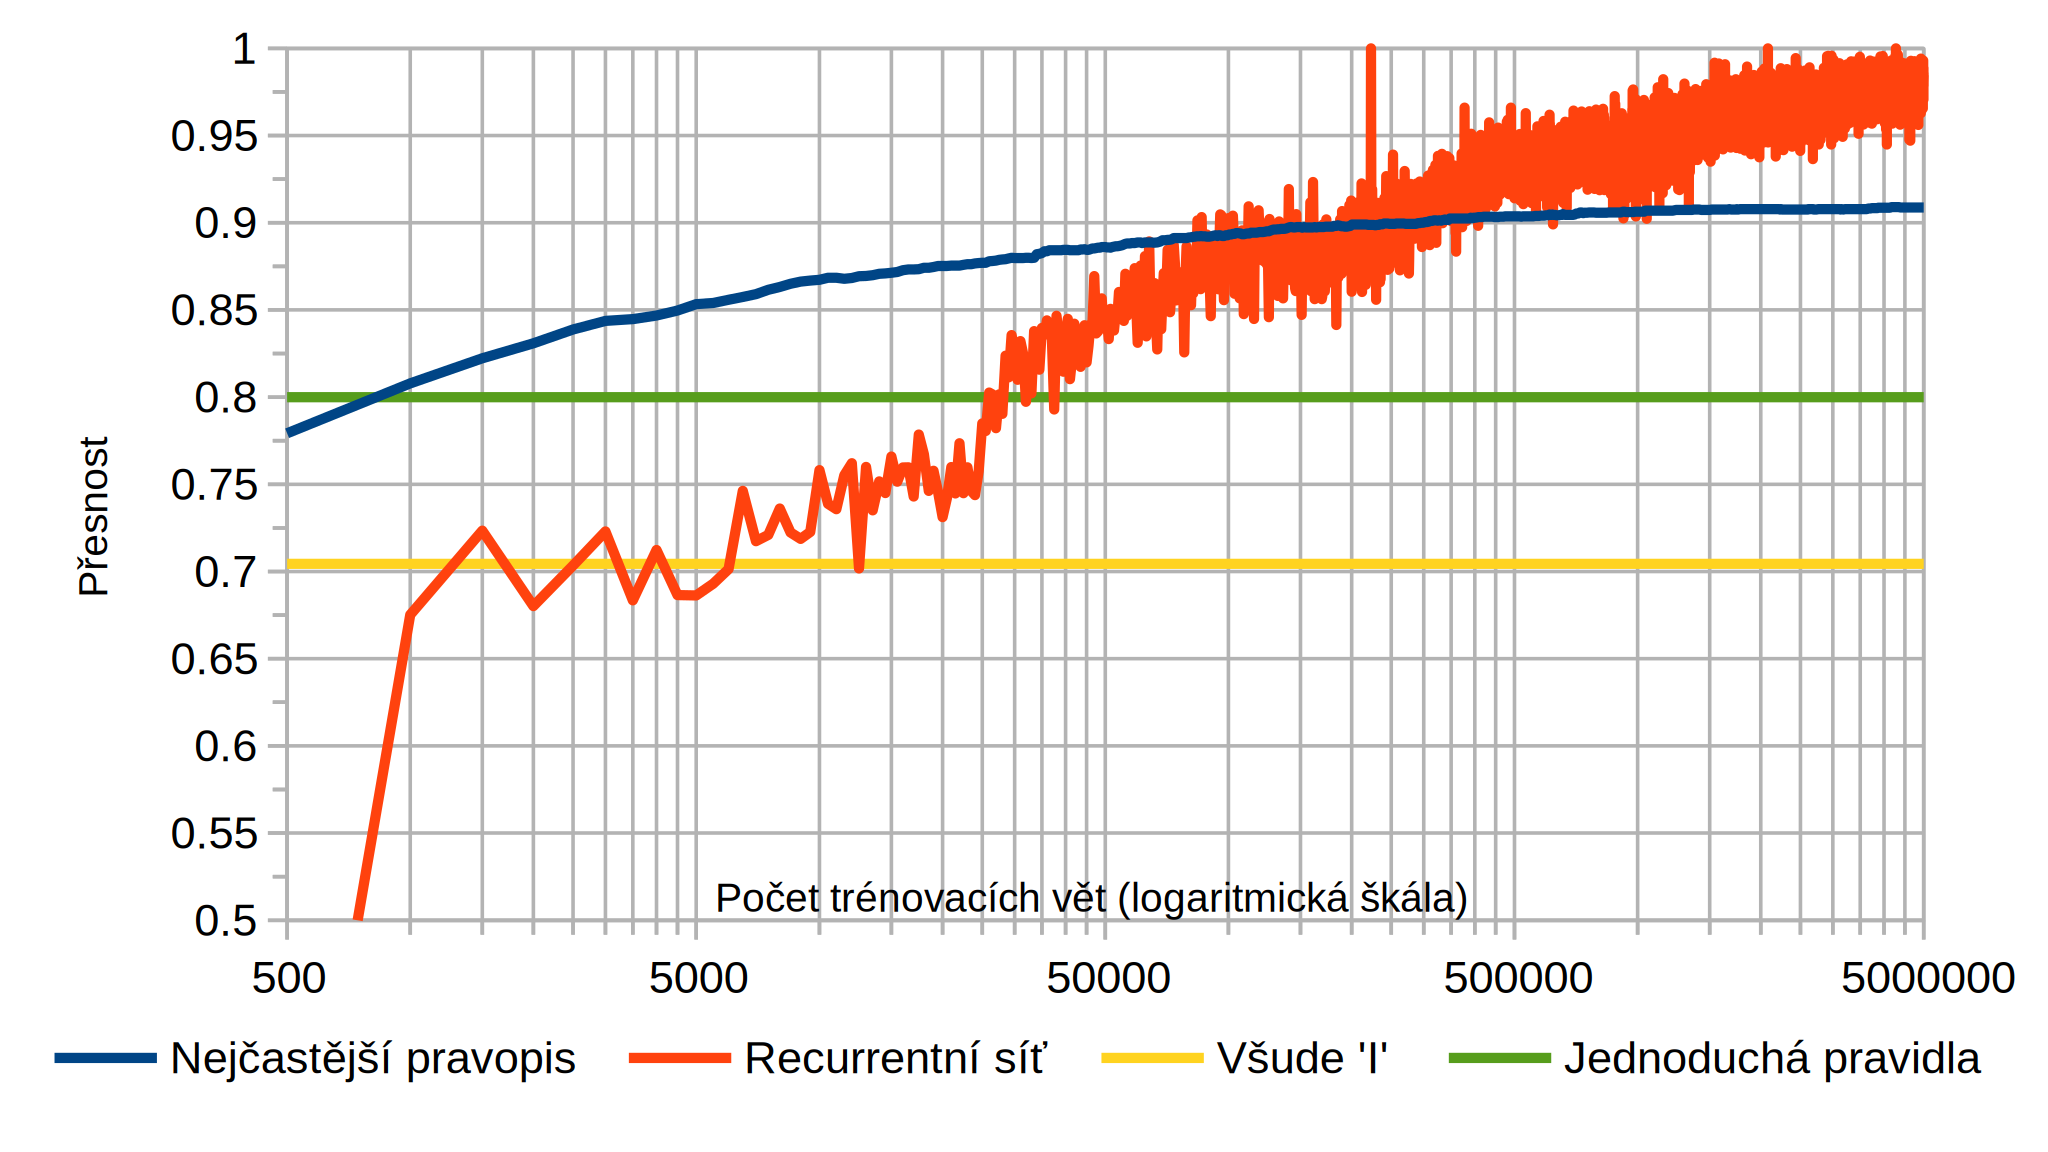
\includegraphics[scale=.5]{./img/spelling_learning_curve_cs.pdf}
    \end{columns}}

\end{frame}

% ----------------------------------------------------------------------------
